\chapter{Experiments and Results}
\label{AER}
This section presents the various experimental results obtained. 

\section{Graph Behavior}
\Cref{tab:results:graph_behavior} qualitatively elaborates how a change in parameter value changes the shape and population level of the populations. 
\Cref{fig:created:a_good_curve_linear} is used as a “ground truth”.  
The default values for \Cref{fig:created:a_good_curve_linear} can be found in \Cref{tab:appendixE:a_good_curve}. 
The default value can also be found in the “Parameter” column, while the tested value is found in the “Tested Value” column. 
Each parameter was individually changed to a higher and lower value from the reference value, and the visual changes are noted in \Cref{tab:results:graph_behavior}. 
This table is not meant to be exhaustive, cover edge cases, or extreme cases, or cover every exact detail and change in the population graph. 
The table is rather to give an idea of how a change in parameter influences the graph shape, such as the rate of resource depletion, maximum number of bacteria and phages, and change in peak time. 

\begin{table}
    \footnotesize
    \centering
    \begin{tabularx}{\textwidth}{l l X}
        \toprule
        \textbf{Parameter} & \textbf{Tested Value} & \textbf{Behavior Description} \\
        \midrule
        $R$ (400) & 500 & More uninfected and infected bacteria, slightly more phages. Resources last longer before being depleted. \\
         & 300 & Slightly less uninfected and infected bacteria, slightly less phages, and earlier resource depletion. \\

        \midrule
        $U$ (50) & 70 & Slightly more phages and uninfected and infected bacteria. Resources are depleted faster. \\
         & 30 & Less uninfected and infected bacteria, slower resource depletion, not all resources used, slightly less phages are created. \\

        \midrule
        $P$ (10) & 20 & Less resources consumed, less bacteria created, bacteria population peaks earlier, slightly less phages.\\
         & 5 & Resources are consumed faster, more uninfected, infected, and phages. Bacteria population peaks at a later time. \\

        \midrule
        $\tau$ (2.14) & 3 & Bacteria population peaks later, with a plateau in population after peaking before infections take place. Phages population is still growing. Infected bacteria peak significantly later. Significant increase in bacteria population. \\
         & 0.5& Barely any resource consumption, little bacteria growth and uninfected, more phages created, phages reach final value very fast. Bacteria population peaks very early. \\

        \midrule
        $\omega^i$ (0) & 15 & Slightly more bacteria are created, resource replenish after bacteria die out. Resources are not depleted and regrow after bacteria die out. Slightly more bacteria are created. \\

        \midrule
        $e$ (0.03) & 0.1 & Faster resource depletion, sharper decline in uninfected, slightly less infected bacteria and phages. Drop in uninfected bacteria happens faster. Bacteria sum peak is sharper and happens earlier. \\
         & 0.01 & Not all resources are consumed, slightly more bacteria are created. \\

        \midrule
        $v$ (1.2) & 1.8 & Resources are finished faster, significantly more uninfected and infected bacteria. Bacteria population peaks earlier, and there are more phages. Peak of the bacteria curve is more sharp and less rounded. \\
         & 1 & Less phages and bacteria are created, not all resources are consumed, bacteria population peaks a tiny bit earlier.\\

        \midrule
        $K$ (10) & 500 & Not all resources are consumed, less bacteria and phages are created, earlier bacteria peak.\\
         & 1 & Faster resource depletion and sudden stop instead of gradual slowdown, more uninfected, infected, and phages create. \\

        \midrule
        $r$ (0.01) & 0.1 0.1& Less resource consumption, significantly less bacteria and phages, earlier peak in bacteria.\\
         & 0.001 & Faster resource consumption rate, significantly more bacteria and phages, delay in uninfected and infected peak, sharp uninfected bacteria peak, sharp bacteria sum peak with a mini plateau before dropping. \\

        \midrule
        $\beta$ (20) & 50 & Significantly more phages and significantly less bacteria, earlier bacteria peak, less resources consumed. Steeper fall in uninfected bacteria, steeper rise in infected bacteria. \\
         & 10 & Faster resource consumption, significantly more uninfected, less phages, sharper uninfected and total bacteria peak, total bacteria population has a plateau before falling. \\

        \midrule
        $\omega^o$ (0) & 0.02 & Faster resource depletion, more bacteria created, later peak in bacteria population. Faster decrease in uninfected bacteria, slightly less phages created, with a gradual decrease in phages post peak. \\

        \bottomrule
    \end{tabularx}
    \caption{
        A table that compares how moving one individual parameter value up or down relative to \Cref{fig:created:a_good_curve_linear} changes the general shape of the curve. 
        Reference parameter values used to compare the produced curves are included in the parentheses, taken from \Cref{tab:appendixE:a_good_curve}. 
    }
    \label{tab:results:graph_behavior}
\end{table}

\section{SOBOL Sensitivity Analysis Results}
\label{sec:SOBOL_sensitivity_analysis_results}

\Cref{fig:created:SOBOL_final_no_wi_wo} shows the impact that the parameter had on the final value of the population at $t=15$ for a $1\times 1\times 1$ system. 
\Cref{fig:created:SOBOL_peak_no_wi_wo} shows the impact that the parameter had on the peak population count, using the 95\% rule. 
\Cref{fig:created:SOBOL_peak_time_no_wi_wo} shows the impact that the parameter had on the time of the peak, using the 95\% rule. 

The parameters that were tested include all the parameters listed in the basic Golding model, except for Uninfected Bacteria, $M$, washin, and washout. 
Uninfected Bacteria was left out as it doesn't make sense to start with infected bacteria to the system, and infected bacteria go from state to state in a constant uniform manner. 
$M$, the number of stages that the infection goes through, can not be tested as $M$ hard-codes the array size of the uninfected bacteria before the simulation framework starts. 
As such, it is not possible to change $M$ without rerunning the program from the very start. 
The washin rate and washout rate consistently had the largest influence on the final, peak value, and time of peak value, using the 95\% rule. 
Washin and washout significantly skewed the results and analysis and warrants an analysis without washin and washout. 
The results for a SOBOL analysis with washin and washout can be found in \nameref{sec:AppendixF:sobol_analysis_with_washin_and_washout}. 


\subsection{Final Value Results}
\subsubsection{Resources}
The final value for the resources depended heavily on the initial Resource concentration. 
There weren't many interactions with other parameters because $ST \gg S1$. 
$e$ had little influence on the system despite $e$ acting as the link between the resources and bacteria and directly controlling the rate of resource consumption. 
$\tau$ had a larger influence in the final resource value than $e$. 
\subsubsection{Phages}
The final phage population depended on $r$ the most, with $\beta$ as the second most important parameter influencing the final population value. 
The other parameters had little to no influence on the final phage population levels. 
\subsubsection{Total Bacteria}
The final total bacteria population depended mostly on $\beta$, but via many second or higher interactions as noted by $ST \gg S1$. 
The final population depended heavily on many higher order interactions with Resources, $\tau$, and $e$. 
Resources, $\tau$ and $e$ was responsible for about 25\% of the sensitivity to the output each. 

\subsection{Peak Value Results}
\subsubsection{Phages}
The SOBOL peak value plot is basically the same as the final value. 
Similar to the Final Value Analysis, the phage max value is highly dependent on the value of $r$ and $\beta$. 
\subsubsection{Total Bacteria}
The total bacteria peak value analysis has similar plot shape. 
$\beta$ still has the largest bar graph, but instead of $ST$ and $S1$ being equal to 1 and 0.28 like in the final value, the sensitivity value is only 0.54 and 0.16 respectively. 
Every parameter plays some influence on the output, but with higher order interactions as for all parameter inputs, $ST > S1$. 

\subsection{Time of Peak Value Results}
\subsubsection{Phages}
With the time of peak value, $\tau$ becomes the most important parameter for determining the final phage value and $r$ and $\beta$ less so. 
\subsubsection{Total Bacteria}
$\beta$ and $\tau$ are the two most important factors in determining the time of peak for the total bacteria. 
The only parameter that does not influence the time of peak is $e$, otherwise every parameter influences the time at which the bacteria population peaks. 

\begin{figure}[ht!]
    \centering
    \begin{subfigure}{0.32\linewidth}
        \centering
        \captionsetup{width=1\linewidth}
        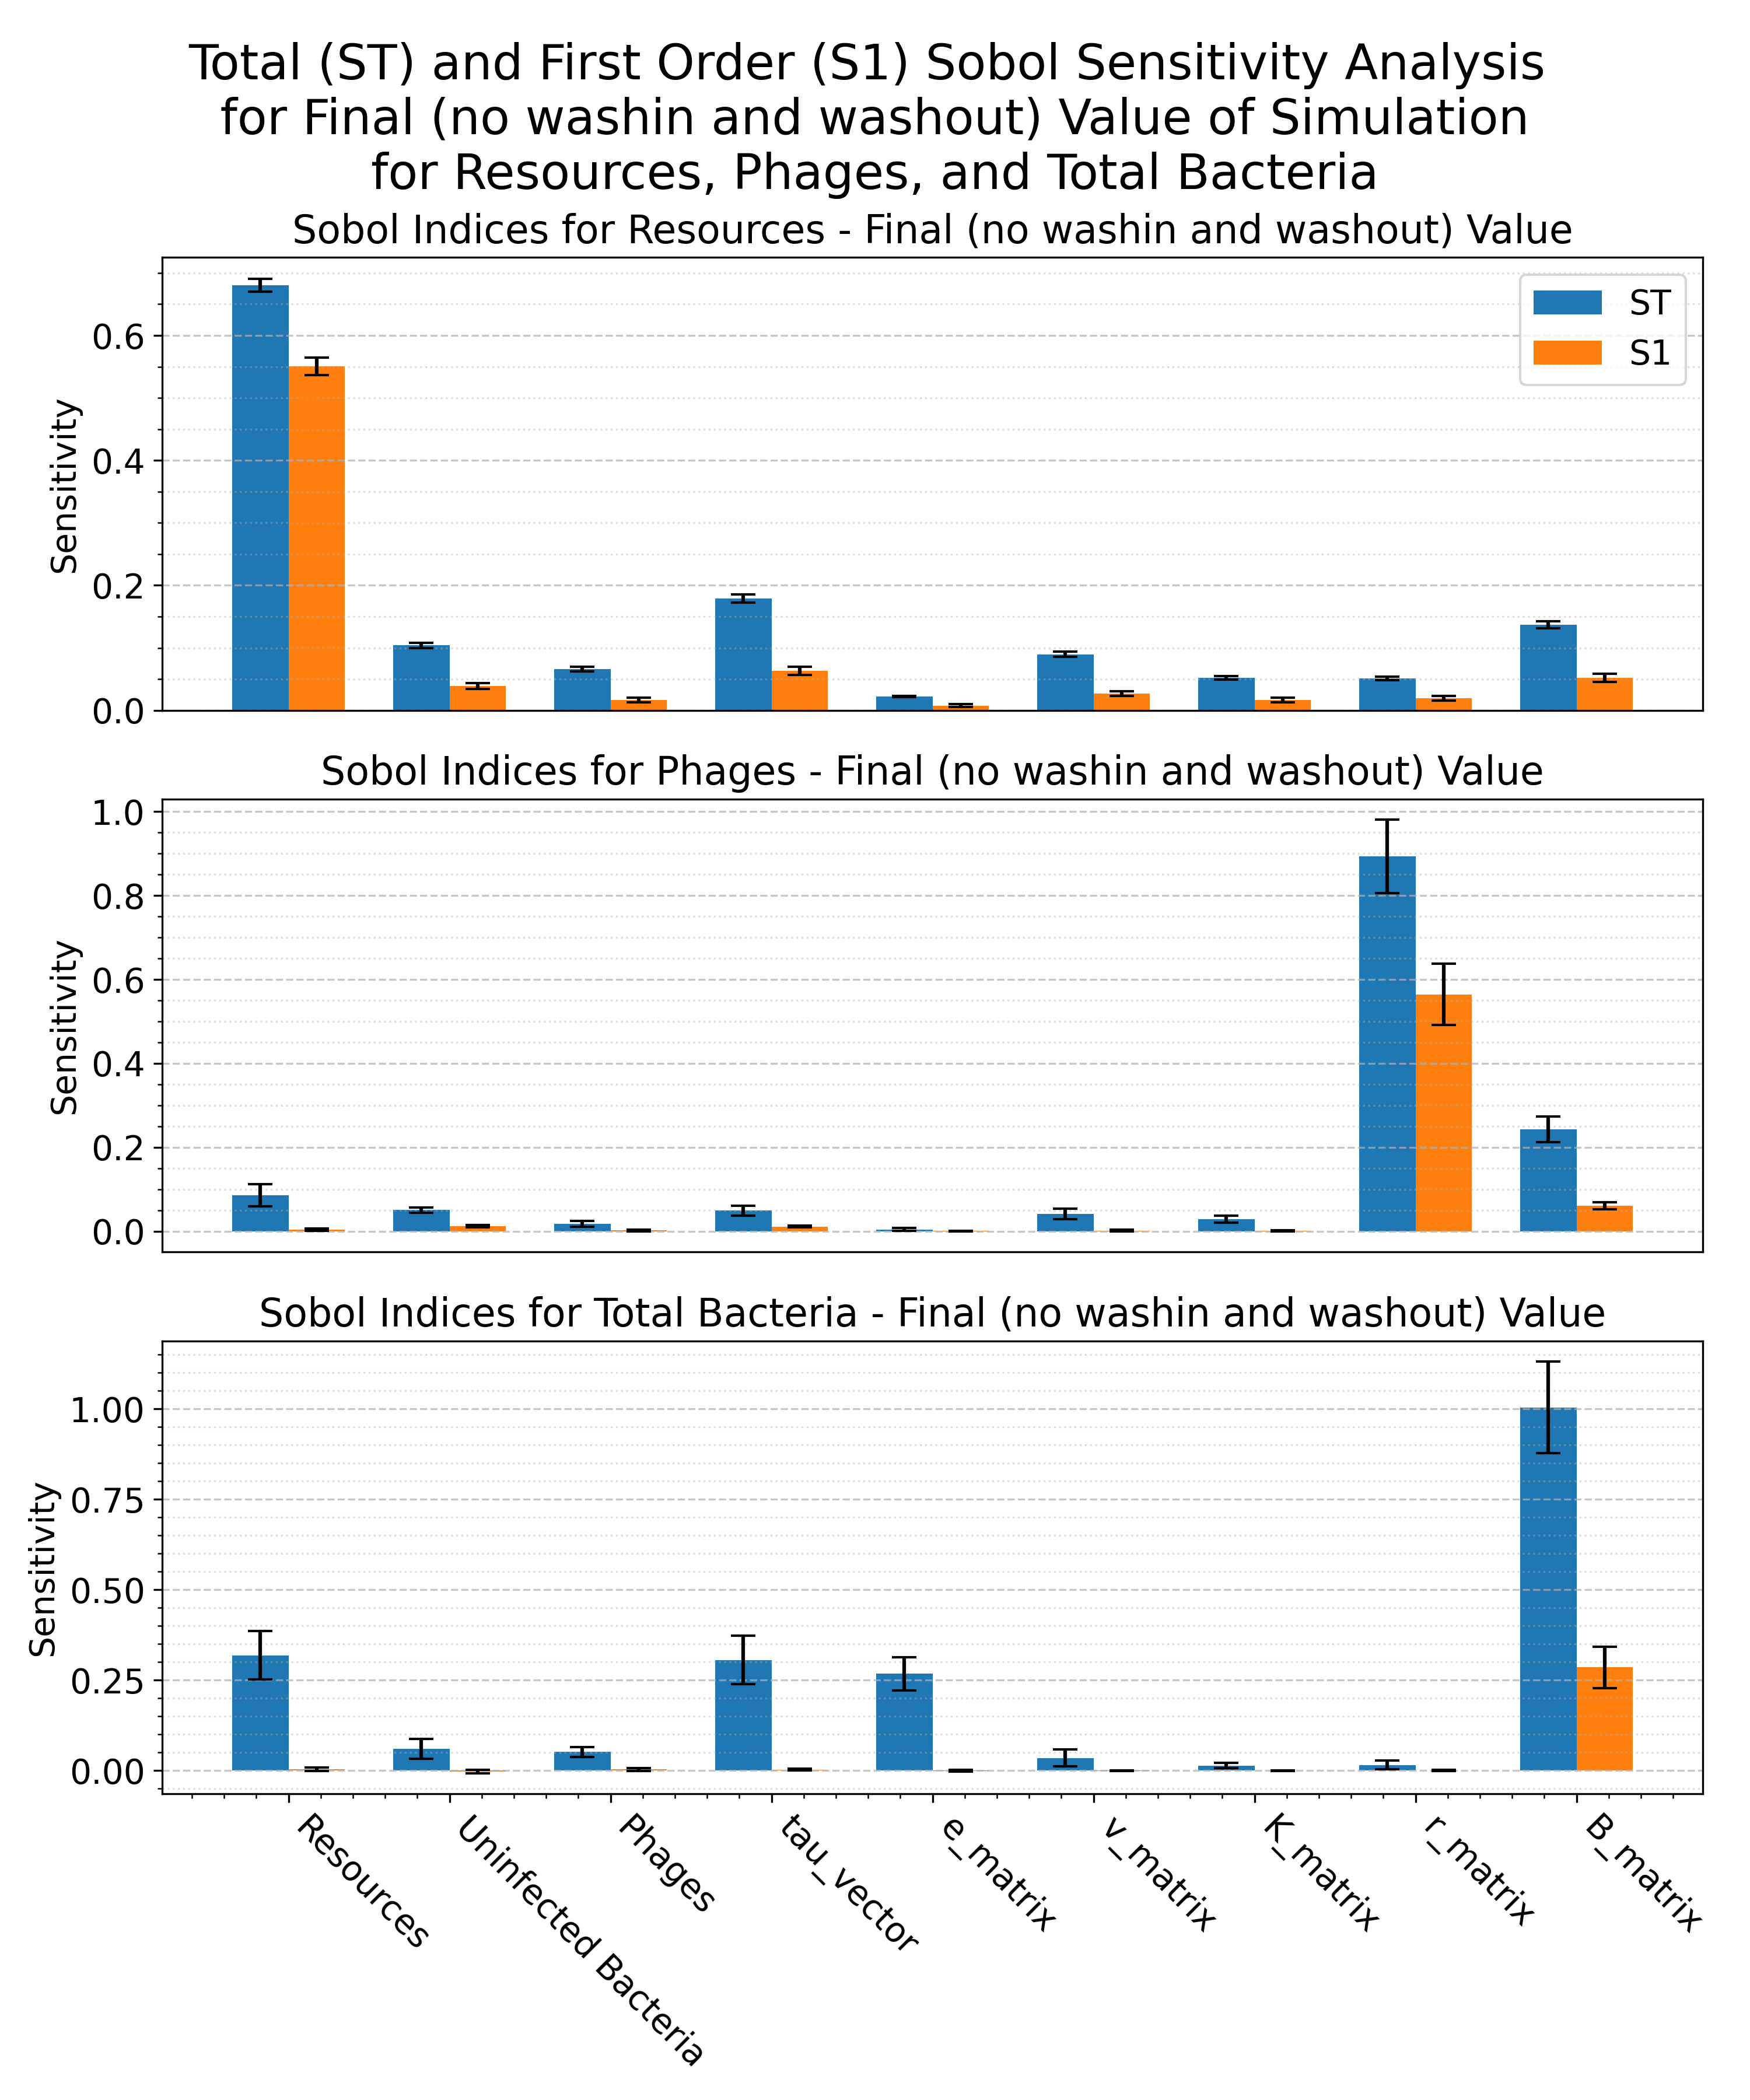
\includegraphics[width=\linewidth]{Plots/Created/SOBOL/SOBOL_analysis_1749708738_Final_(no_washin_and_washout).png}
        \caption{
            Final value, no washin and washout. 
        }
        \label{fig:created:SOBOL_final_no_wi_wo}
    \end{subfigure}
    \hfill
    \begin{subfigure}{0.32\linewidth}
        \centering
        \captionsetup{width=1\linewidth}
        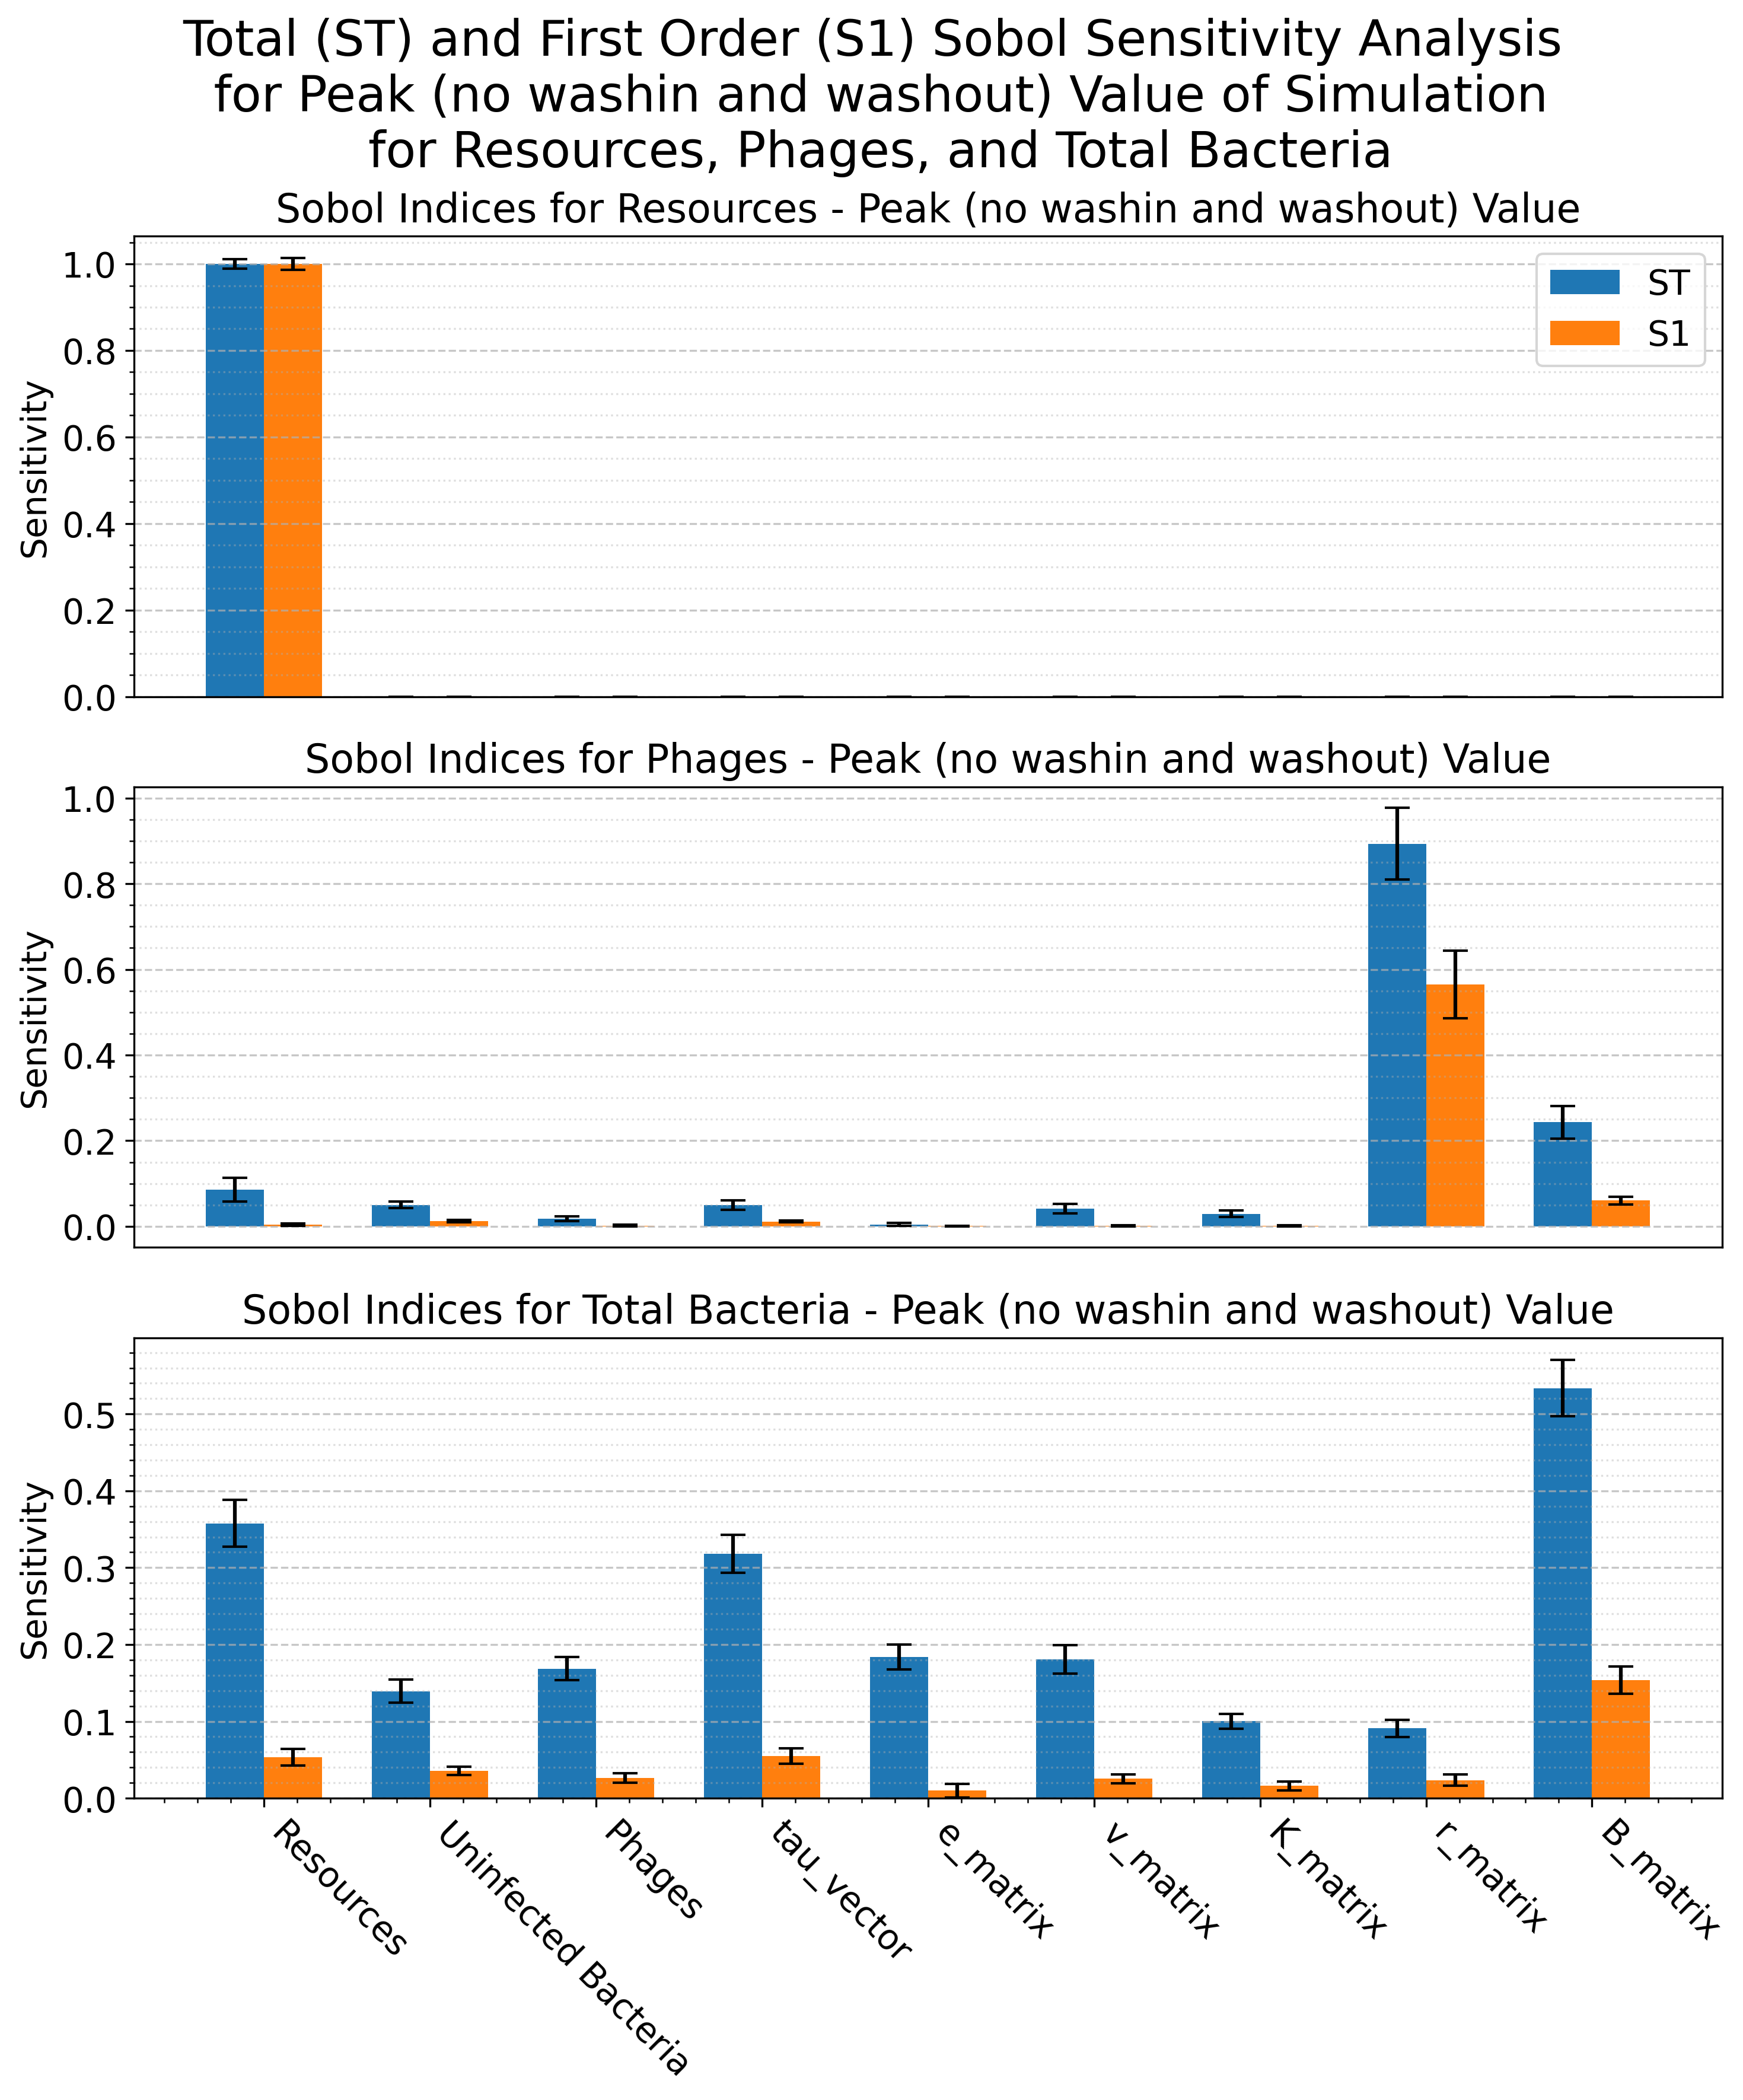
\includegraphics[width=\linewidth]{Plots/Created/SOBOL/SOBOL_analysis_1749708738_Peak_(no_washin_and_washout).png}
        \caption{
            Peak population value, no washin and washout. 
        }
        \label{fig:created:SOBOL_peak_no_wi_wo}
    \end{subfigure}
    \hfill
    \begin{subfigure}{0.32\linewidth}
        \centering
        \captionsetup{width=1\linewidth}
        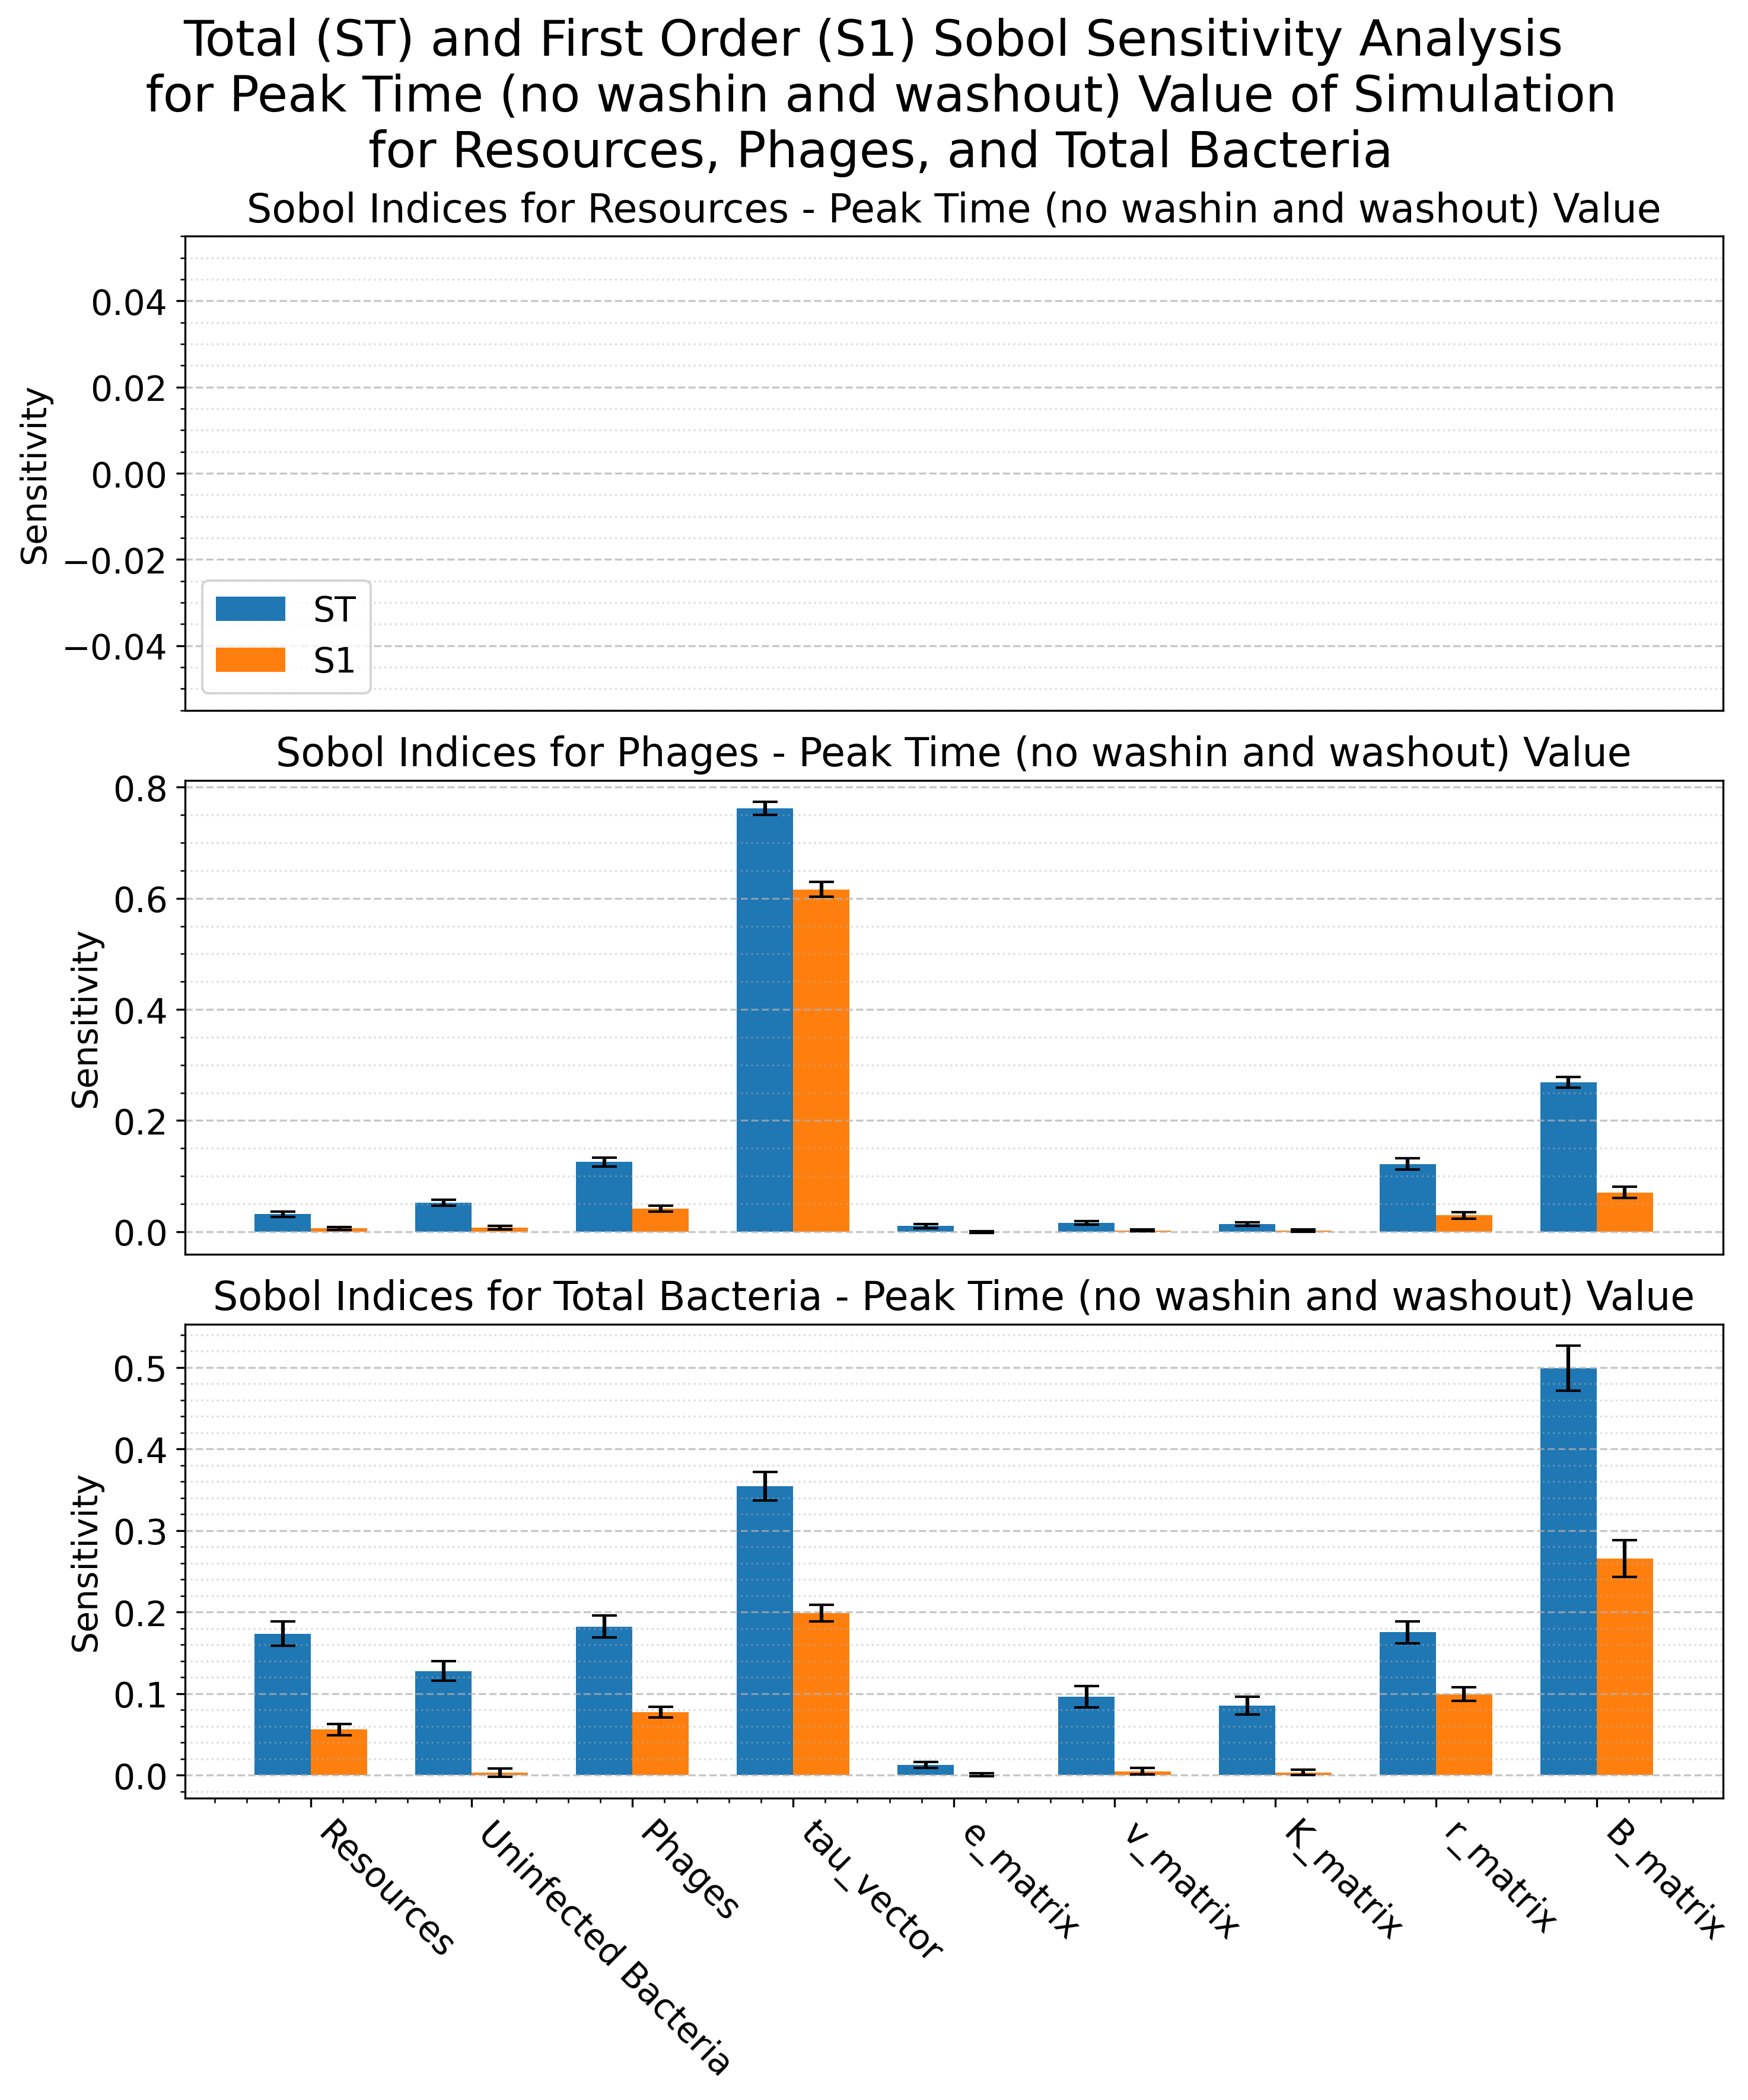
\includegraphics[width=\linewidth]{Plots/Created/SOBOL/SOBOL_analysis_1749708738_Peak_Time_(no_washin_and_washout).png}
        \caption{
            Time of peak value, no washin and washout. 
        }
        \label{fig:created:SOBOL_peak_time_no_wi_wo}
    \end{subfigure}
    \caption{
        SOBOL analyses for the final, peak, and time of peak value, without a washin and washout rate.
        The input value ranges to test each parameter used for this SOBOL test can be found in \Cref{tab:appendixE:SOBOL_analysis_values}, except washin and washout was set to 0. 
    }
    \label{fig:created:SOBOL_no_wi_wo}
\end{figure}

\section{Initial Value Analysis Results}
\label{sec:results:initial_value_analysis}

\Cref{fig:created:initial_value_analysis_UB_50_500_a_good_plot_2} and \Cref{fig:created:initial_value_analysis_UB_50_500_a_good_plot} illustrate how varying the initial uninfected bacteria population from 1 to 500 (using 100 different starting values) affects the dynamics and time of peak population of phage and total bacteria populations using the 95\% rule. 

\Cref{fig:created:initial_value_analysis_UB_50_500_a_good_plot_2} replicates Figure 1 of \citet{mullaExtremeDiversityPhage2024} perfectly. 
As the initial bacteria population increases, the time to reach the phage and bacteria sum peak decreases, following $y = -0.8648\cdot ln(x) + 9.7911$ and $y = -1.0056\cdot ln(x)+7.7626$, with $R^2=0.9800, 0.9988$ respectively. 

\Cref{fig:created:initial_value_analysis_UB_50_500_a_good_plot} on the other hand shows different behavior. 
As the initial bacteria population decreases from 500 to 100, the same behavior in \Cref{fig:created:initial_value_analysis_UB_50_500_a_good_plot_2} is noticed.
There is a change in behavior at 100 and less initial uninfected bacteria. 
Instead of following the predicted line like in \Cref{fig:created:initial_value_analysis_UB_50_500_a_good_plot_2}, the curve for the phages suddenly decreases, following a quadratic like curve. 
The bacteria on the other hand plateau before starting to increase again. 
Both curves resemble a spoon-like shape. A straight handle with a “bowl” to hold the liquid. 
The fitted curves follow $y = -0.1292\cdot ln(x) + 10.1462$ and $y = -0.6234\cdot ln(x)+6.9602$, with $R^2=0.5406, 0.9206$ respectively. 
Despite the large bacteria sum $R^2$ value, the fitted curve does not fit the data. 

\begin{figure}
    \centering
    \begin{subfigure}{1\linewidth}
        \centering
        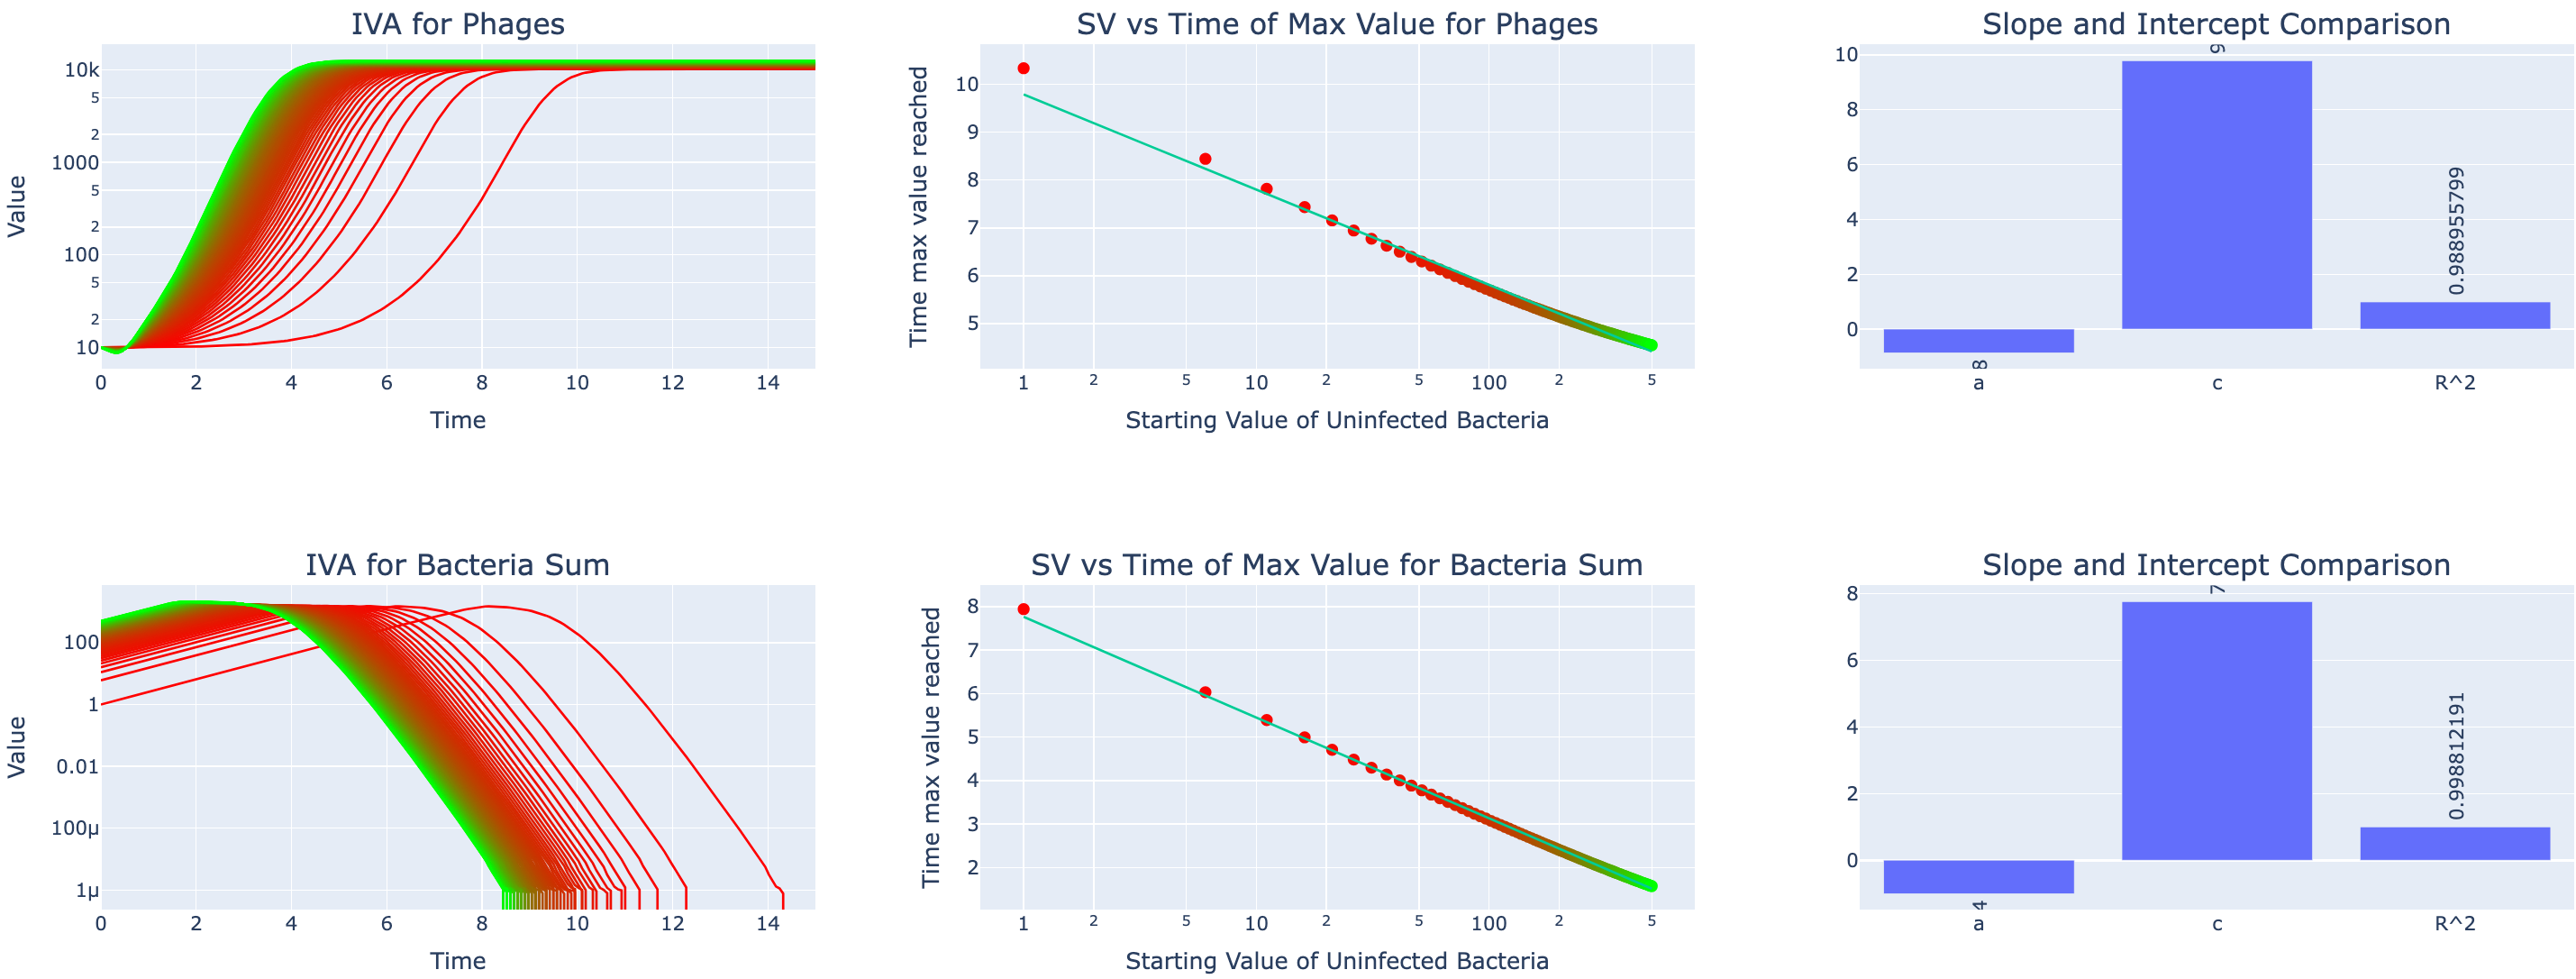
\includegraphics[width=\linewidth]{Plots/Created/IVA/initial_value_analysis_UB_50_500_a_good_plot_2.png}
        \caption{
            IVA for \Cref{tab:appendixE:a_good_curve_2}. 
            Replicates Figure 1 of \citet{mullaExtremeDiversityPhage2024}. 
            The system is adsorption limited \cite{mullaExtremeDiversityPhage2024}. 
        }
        \label{fig:created:initial_value_analysis_UB_50_500_a_good_plot_2}
    \end{subfigure}
    \hfill
    \begin{subfigure}{1\linewidth}
        \centering
        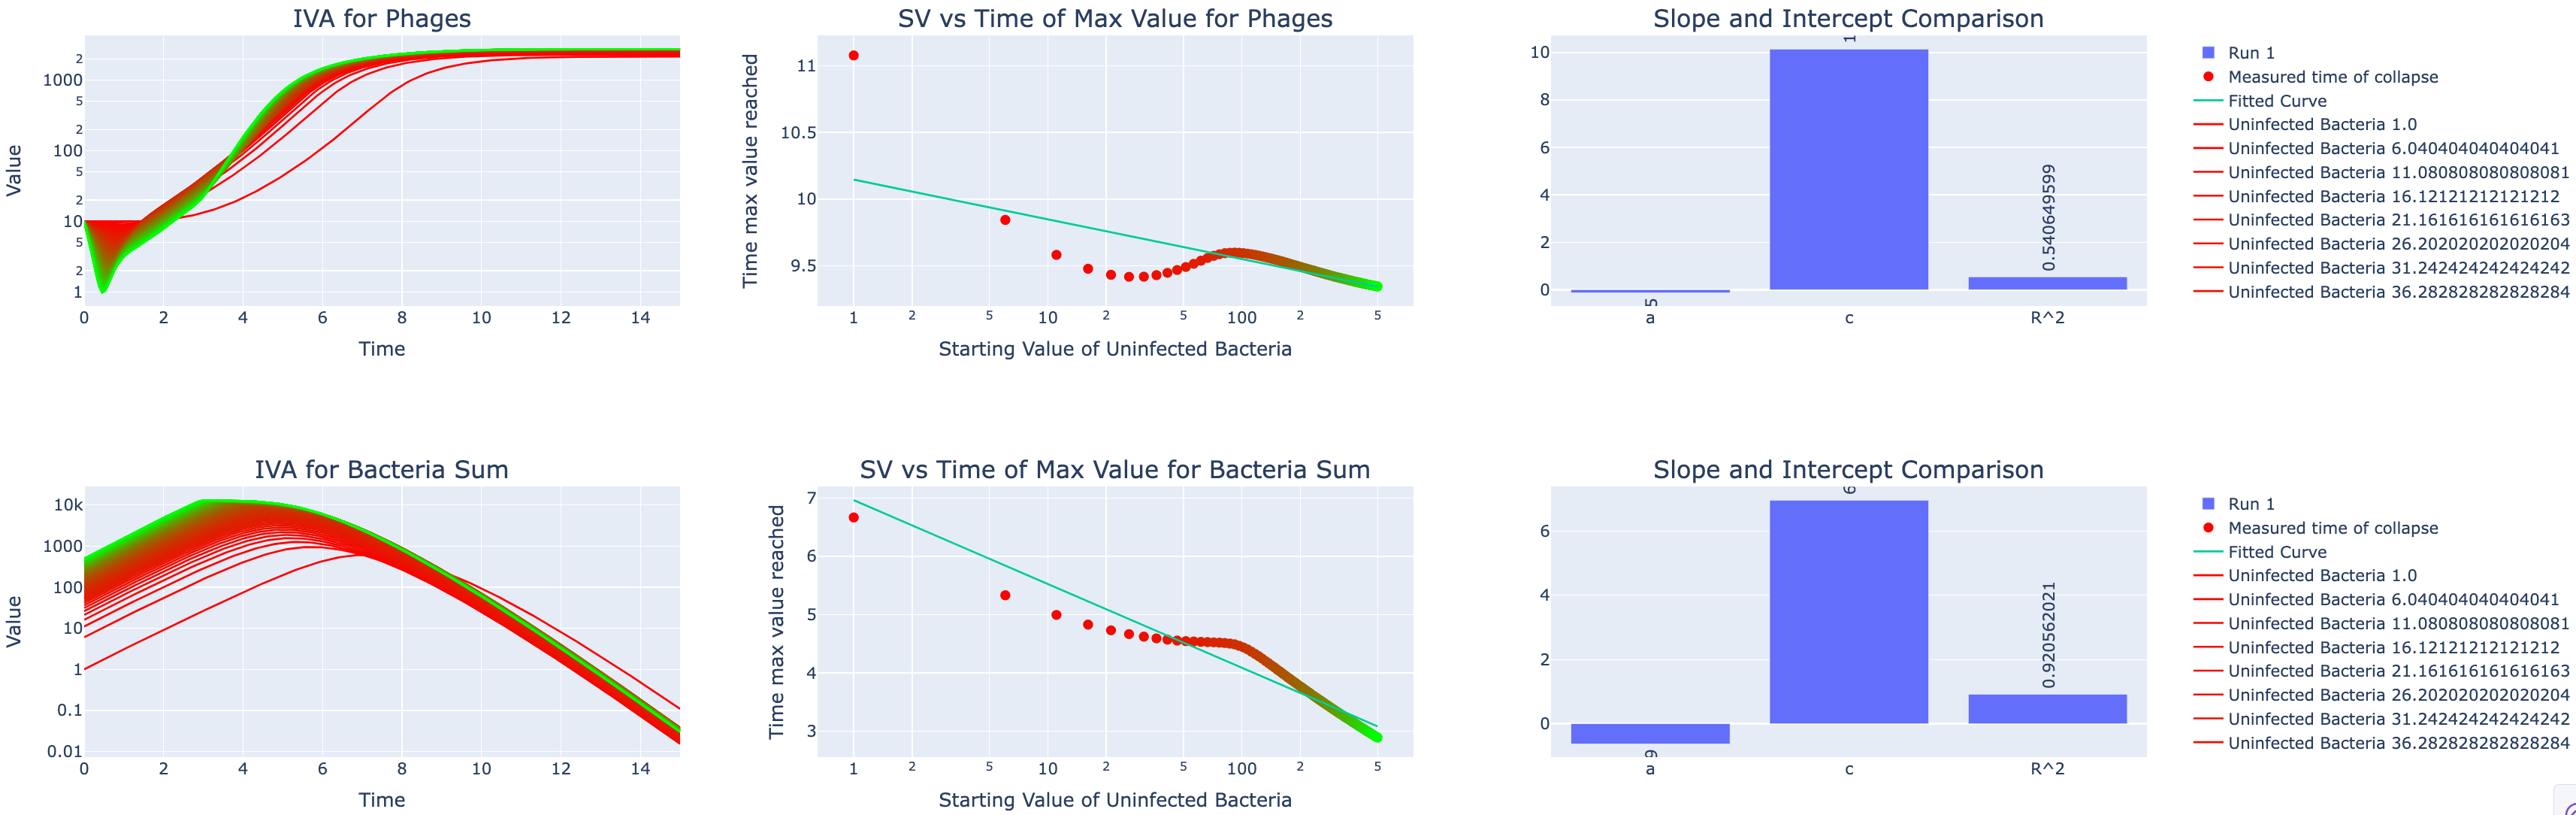
\includegraphics[width=\linewidth]{Plots/Created/IVA/initial_value_analysis_UB_50_500_a_good_plot.png}
        \caption{
            IVA for \Cref{tab:appendixE:a_good_curve}. 
            For uninfected bacteria less than 100, the phage-bacteria interaction is resource limited. 
        }
        \label{fig:created:initial_value_analysis_UB_50_500_a_good_plot}
    \end{subfigure}
    \caption{
        Varying initial Uninfected Bacteria concentration, from 50 to 500, with 30 unique values tested over two different instances of "good" curves. 
        Even with two "good" curves, even varying the default parameter values a tiny bit can have a large influence on how changing the initial bacteria concentration can have an influence on the dynamics of the system, changing the behavior of the peak time. 
        The default values for Figure a) and b) can be found at \Cref{tab:appendixE:a_good_curve} and \Cref{tab:appendixE:a_good_curve_2}. 
    }
\end{figure}

\section{Phase Portrait}
\label{sec:results:phase_portrait}
\Cref{fig:created:phase_portrait_resources_245-265_phages_25-26} shows a phase portrait varying the initial resource and phage concentration. 
For phages that start above 25.98, the phage population can proliferate (until the washout would eventually remove the phages). 
For phage populations that start below 25.98, the washout removes the phages before the phages had time to infect and kill the bacteria. 
Both regions of phages exhibit consistent behavior, of either going to 0 or proliferating. 
If the phage population started at exactly 25.98, if the initial resources was 260 or above, the phages died out. 
If the initial resources was 255 or below, the phages would proliferate. 
Expanding on these results by simulating more initial values creates \Cref{fig:created:phase_portrait_resources_phage}. 
The initial resource values span from 1 to 500, and the initial phage values range from 25.5 to 26.5, each with 100 unique values sampled.
Each cell is a unique set of initial conditions. 
If the phages proliferated for that condition, the box is colored red. 
In this case, proliferated means that the phage population reached at least 2 times the initial condition. 
If the box is white, it means the phages died out before being able to reach 2 times its initial concentration. 
A boundary between the nonproliferating and proliferating phages can be curve-fit following $y=\frac{86.756x}{15.811+x} - 10.241$ with an $R^2$ value of 0.994. 
\Cref{fig:created:phase_portrait_resource_phage_proliferate} zooms into the range $(1-40, 24.2-25)$ for a high detailed view of the behavior happening around initial resources of 10. 
At about resources of 6 or 7, there is a minimum in phage proliferation. 
For initial resource values of 6 or below, as initial resources increase, less phages (although very miniscule changes) are required to proliferate. 
For initial resource values of 7 or above, more phages (although very miniscule changes) are required to proliferate. 

\begin{figure}[]
    \centering
    \begin{subfigure}{0.49\linewidth}
        \centering
        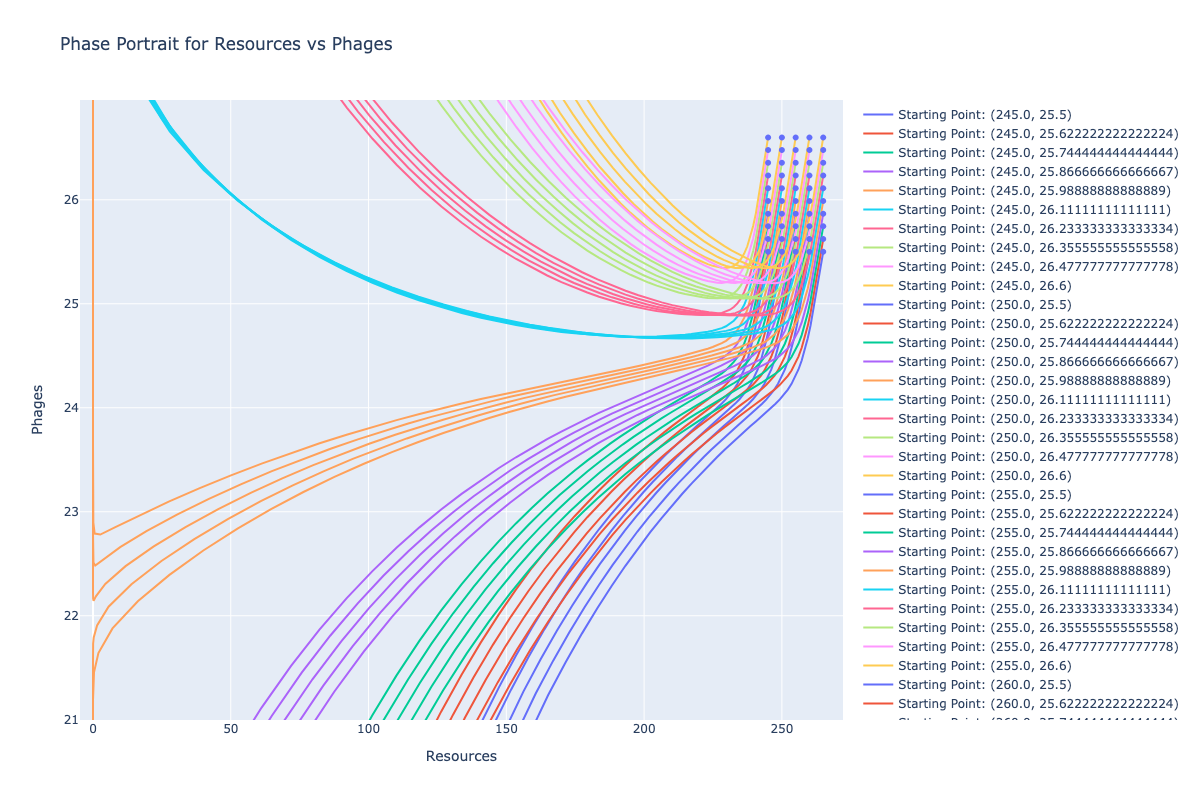
\includegraphics[width=1\textwidth]{Plots/Created/PP/phase_portrait_resources_245-265_phages_25-26.png}
        \caption{
            Zoomed in plot of a phase portrait with varying resource and phage population from 245-265 and 25.5-26.5 respectively. 
            Each row has its own line color. 
            Diverging behavior can be seen for the orange line (phage=25.98). 
        }
        \label{fig:created:phase_portrait_resources_245-265_phages_25-26}
    \end{subfigure}
    \hfill
    \begin{subfigure}{0.49\linewidth}
        \centering
        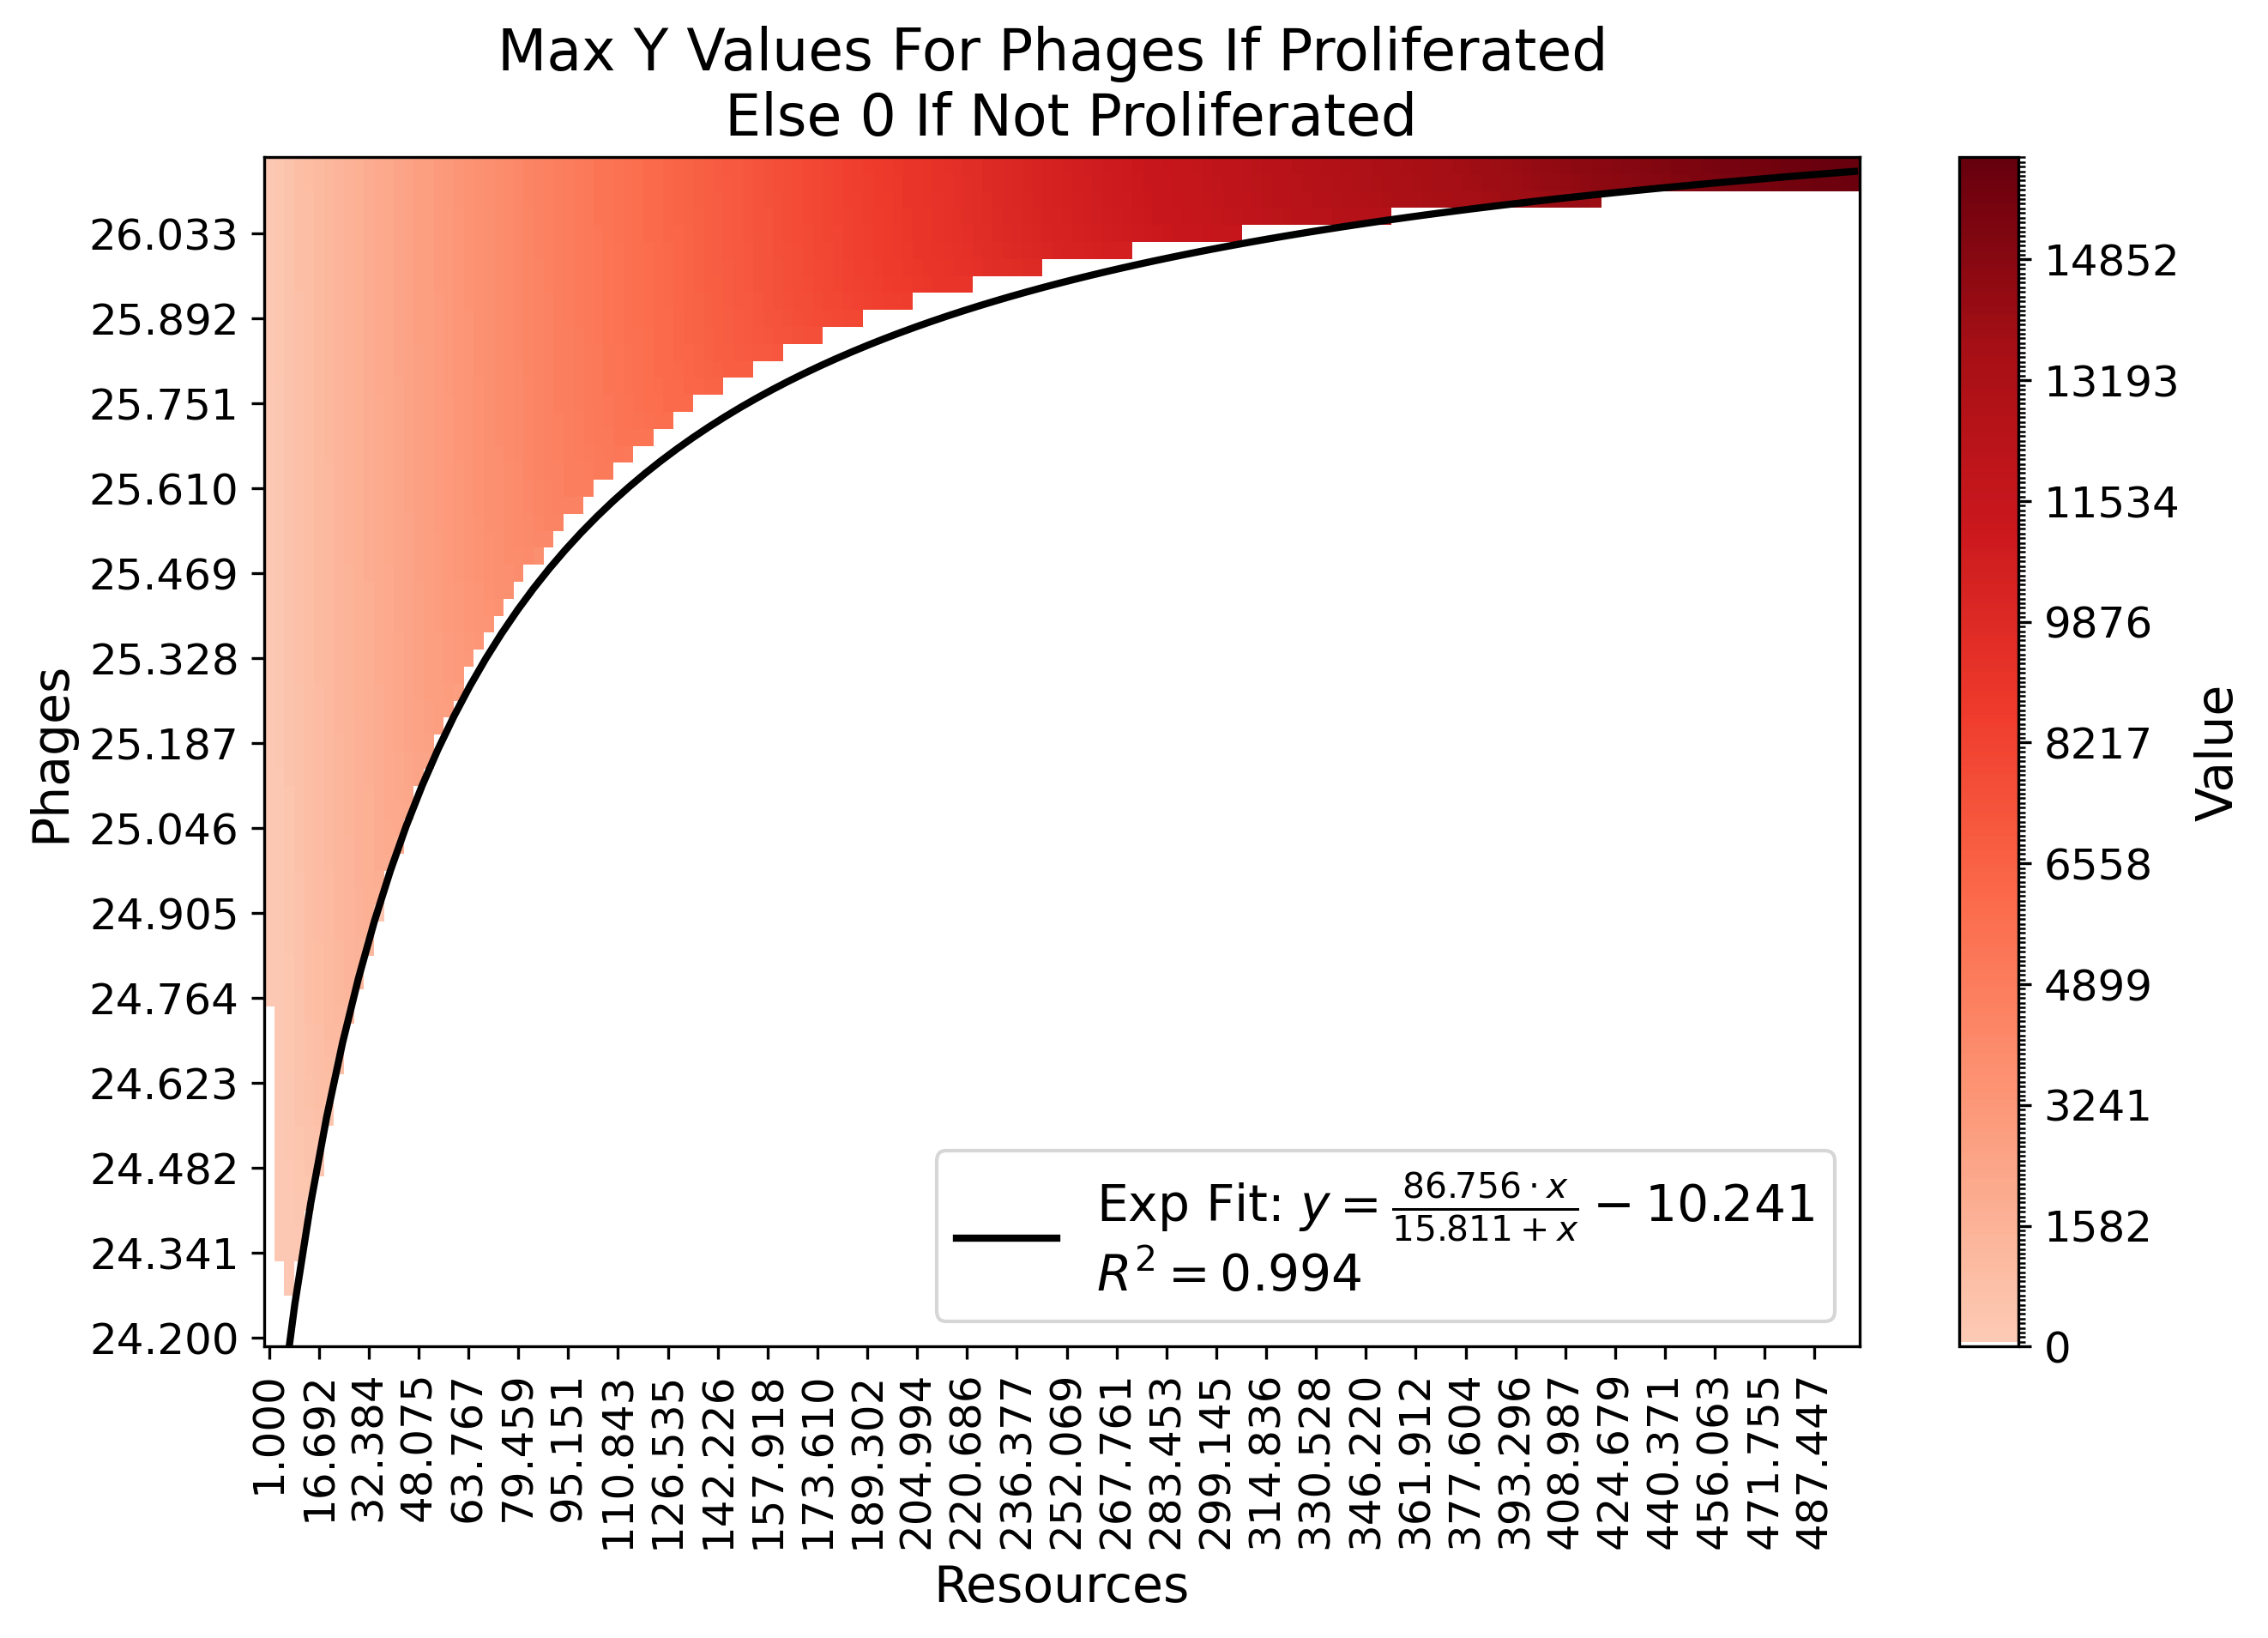
\includegraphics[width=\linewidth]{Plots/Created/PP/phase_portrait_resources_phage.png}
        \caption{
            Phage population proliferation as a function of initial resource and phage concentrations. 
            While the color appears uniform along the vertical axis, each cell is actually a slightly different value. 
            The phage-resource proliferation boundary follows a fitted Monod equation.
        }
        \label{fig:created:phase_portrait_resources_phage}
    \end{subfigure}
    \hfill
    \begin{subfigure}{0.49\linewidth}
        \centering
        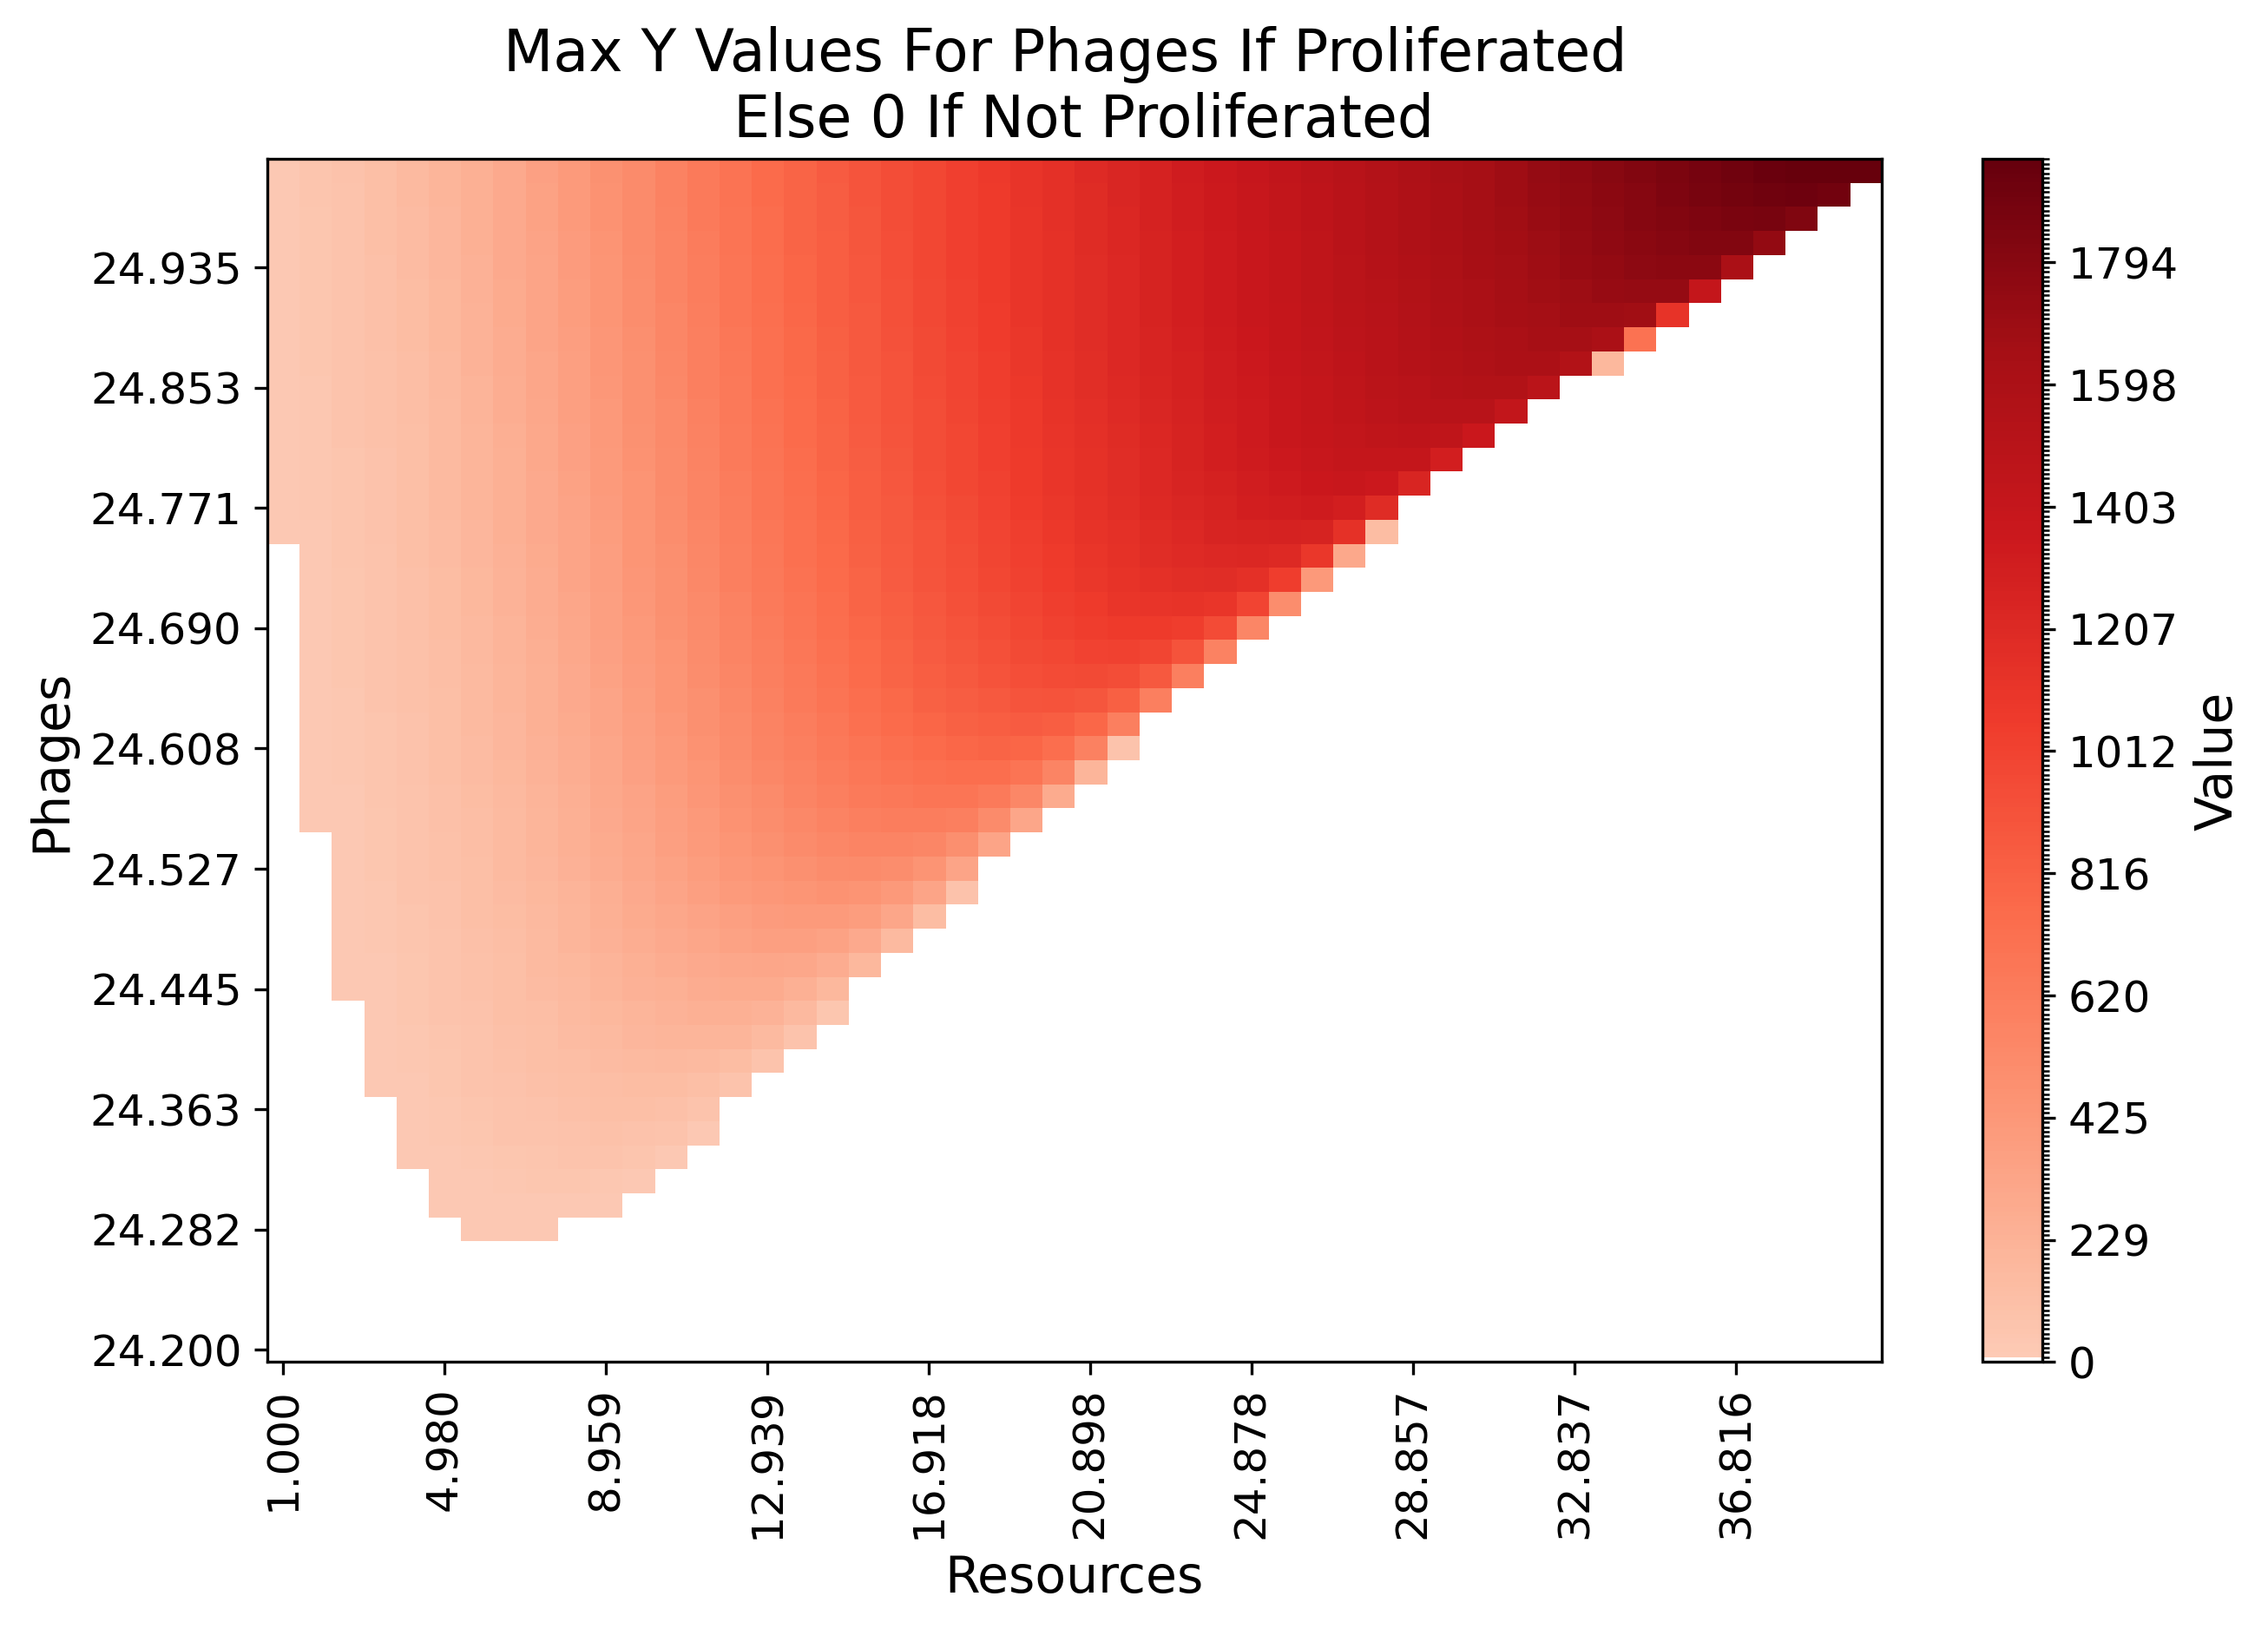
\includegraphics[width=\linewidth]{Plots/Created/PP/phase_portrait_resources_phage_2.png}
        \caption{
            Zoomed in to analyze the regime of behavior change near resources$=10$. 
        }
        \label{fig:created:phase_portrait_resources_phage_2}
    \end{subfigure}
    \caption{
        Varying initial resources and initial phages and the resulting proliferation and fitted proliferation curve. 
        Proliferation is defined as when the phage population reached at least 2 times the initial starting population. 
        This simulation values used can be found in \Cref{tab:appendixE:a_good_curve_2}, but with washout set to 0.02 instead of 0. 
    }
    \label{fig:created:phase_portrait_resource_phage_proliferate}
\end{figure}

\begin{figure}[]
    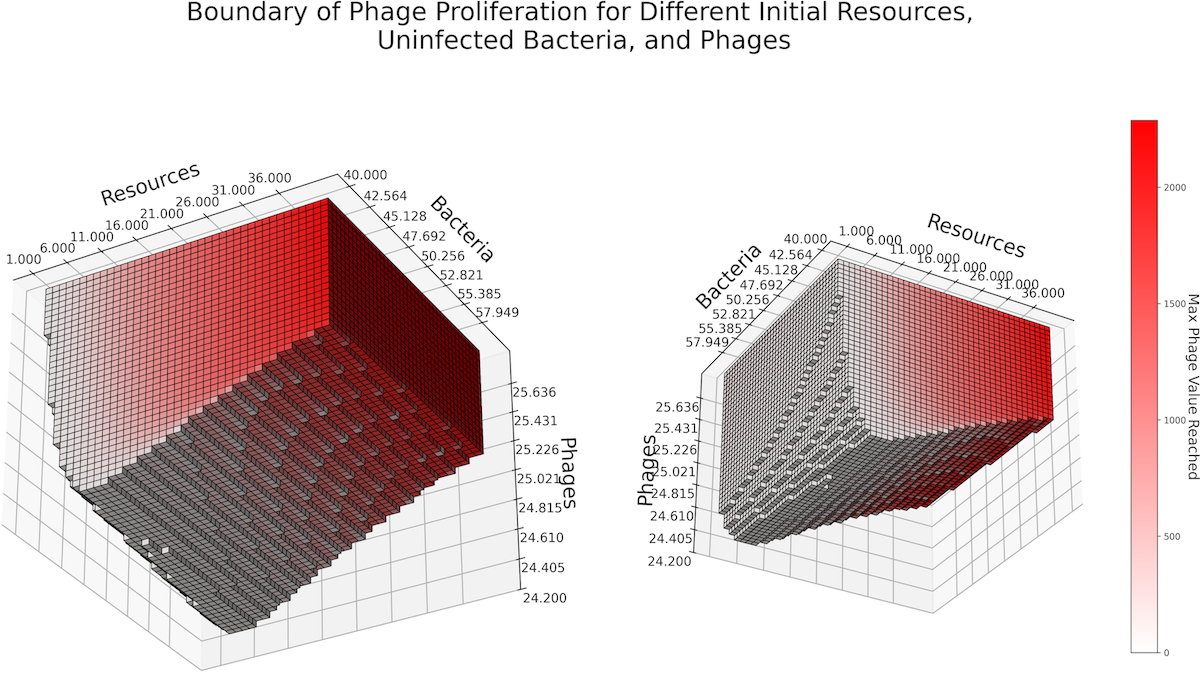
\includegraphics[width=1\textwidth]{Plots/Created/PP/3d_plot_resource_bacteria_phage.png}
    \centering
    \caption{
        3D plot of phage proliferation, dependent on initial resource, uninfected bacteria, and phage population. 
        Color scaling from white to red, color is dependent on the max phage population reached. 
    \label{fig:created:3D_phase_portrait}
    }
\end{figure}

\section{Plotting Parameter Change - $3\times 2\times 3$ Model}
\Cref{fig:created:r_beta_washout_0}, \Cref{fig:created:r_beta_washout_0.02}, and \Cref{fig:created:r_beta_washout_0.05}, show a 7x7 matrix of different $r$ and $\beta$ initial conditions for a $3\times2\times3$ model, and each figure changes the washout rate from 0 to 0.02 to 0.05. 
For each simulation, if $r$ or $\beta$ is equal to a value not equal to $inf$, as identified by the title above each sub-figure, then each value of $r$ or $\beta$ has that value.
All phage initial values started at 10. 
This was specifically chosen to highlight how even though the phage values all start the same, and how two parameter values are controlled, the other parameter values and unequal network topogrpahy has an impact on the population values of the phages. 
If $r$ or $\beta$ is equal to $inf$, then the simulation uses the original data as defined in the IC, vector, and matrix section of the dashboard. 
As a small example for the $3\times 2\times 3$ model, when $r=0.200$, the simulation framework uses $r = \left(\begin{smallmatrix} NaN & 0.200 \\ 0.200 & NaN \\ 0.200 & 0.200 \\ \end{smallmatrix}\right)$ as the input matrix to the ODE model. 
When $r=inf$, the simulation framework uses $r=\left(\begin{smallmatrix} NaN & 0.11695 \\ 0.144459 & NaN \\ 0.11895 & 0.13065 \\ \end{smallmatrix}\right)$ as the data to simulate the interactions with. 
For the cells that don't have an edge between $p$ and $b$ or between $b$ and $r$, the data is represented as $NaN$, short for "Not a Number", \textit{np.NaN}, 

The columns and rows of each figure makes it easy to compare how a change in parameter value affects the curve, while keeping the other parameter the same. 
In $r, \beta, \omega^o=inf, inf, 0$, although not a "good curve" due to limited resource consumption and limited bacterial and phage growth, really shows how the different parameter values for each interaction uniquely affect the growth rate of each agent, especially the phage population (P0=blue, P1=green, and P2=purple). 
Despite all phages starting at the same population level, within the first two or so time units, P1 has less phages than P0 and P2. 
P2 has the fastest initial growth rate, as P2 has the most phages until $t=4$, at which point P1 has a larger phage population. 
P2 reaches its peak population count before P0 or P1, but despite the slower initial growth, P0 and P1 eventually overtake P2 in total phage population. 
P2 also actually reaches its peak before decreasing in population. 
There are trace amounts of infected bacteria at the end of the simulation. 
Since the phage population is reduced by $r_{pb}\cdot(U_b + \sum_{k=1}^M I_{b_k})$, and by specifically choosing the parameter values as used in \Cref{tab:appendixE:complex_model}, behavior that hasn't been seen in a $1\times 1\times 1$ system has been found. 
The complete extinction of the bacteria has been delayed long enough such that at trace amounts, there is phage reduction despite bacteria still existing. 
The peak times for P0, P1, and P2 are $t=6.33, 7.99, 4.52$, a difference of $3.47$ time units. 

Contrast that with the phage population dynamics of that with $r, \beta, \omega^o = inf, 100, 0$, the phage populations do not show interesting dynamics. 
The peak times are more similar and consistent to one another ($t=5.50, 7.01, 6.78$, a difference of $1.51$ time units). 
The phage population curve all appear the same, with slightly slower growth rates. 
There is no crossing of phage populations unlike with $r, \beta, \omega^o=inf, inf, 0$. 

Losing the change in $\beta$ values really affected the dynamics fo the phage population. 
The highlighted example demonstrated the dynamics and influence that multiple agents can have on the final output. 

The top row of \Cref{fig:created:r_beta_washout_0.02} shows how the phages and resources died out relative to the top row of \Cref{fig:created:r_beta_washout_0}. 
Even with a high burst value, the phages could not defeat the pressure from the washout. 
But by changing the $r$ value from $r=0.001$ to $r=0.041$, the phages were able to save themselves and proliferate. 
Using this knowledge, and the information gained from \nameref{sec:results:phase_portrait}, a 3D matrix of phage proliferation can be created. 
\Cref{fig:created:3D_phase_portrait} shows the matrix of proliferation for varying resource, uninfected bacteria, and phage initial conditions. 
The color consistently changes form white to red across the resources axis, and less so across the bacteria or phages axis. 
If spliced along the bacteria axis, there is little difference in the shape of the curve. 
On the underside of the curve, there is some slight variation in color and if the phages proliferated. 
When spliced on the Resource values near 1, there is the decreasing edge of Phage-Bacteria phage proliferation as the initial resource concentration approaches 6. 


\begin{figure}[]
    \centering
    \begin{subfigure}{0.32\linewidth}
        \centering
        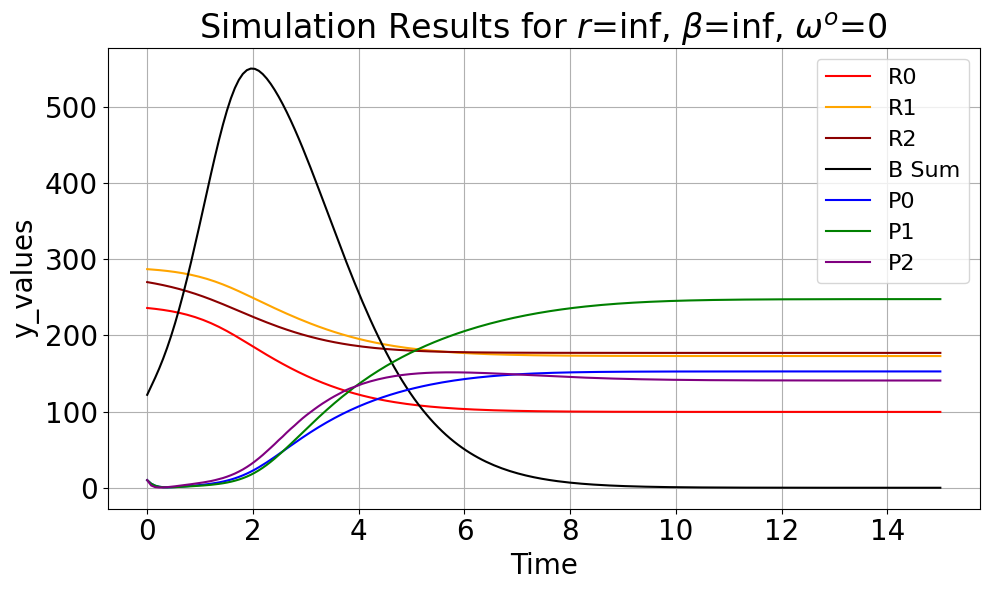
\includegraphics[width=\linewidth]{Images/Plots/Created/UA/r_beta_washout_inf_inf_0.png}
        \caption{
            $r, \beta, \omega^o = inf, inf, 0$, all initial phage condition=10. 
        }
        \label{fig:created:r_beta_washout_inf_inf_0}
    \end{subfigure}
    \begin{subfigure}{0.32\linewidth}
        \centering
        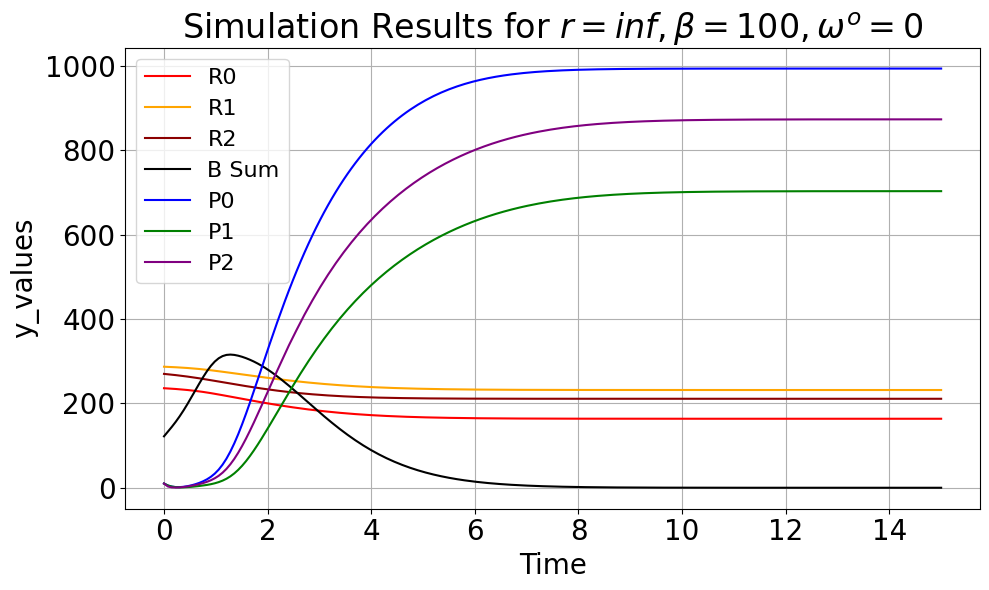
\includegraphics[width=\linewidth]{Images/Plots/Created/UA/r_beta_washout_inf_100_0.png}
        \caption{
            $r, \beta, \omega^o = inf, 100, 0$, all initial phage condition=10. 
        }
        \label{fig:created:r_beta_washout_inf_100_0}
    \end{subfigure}
    \begin{subfigure}{0.32\linewidth}
        \centering
        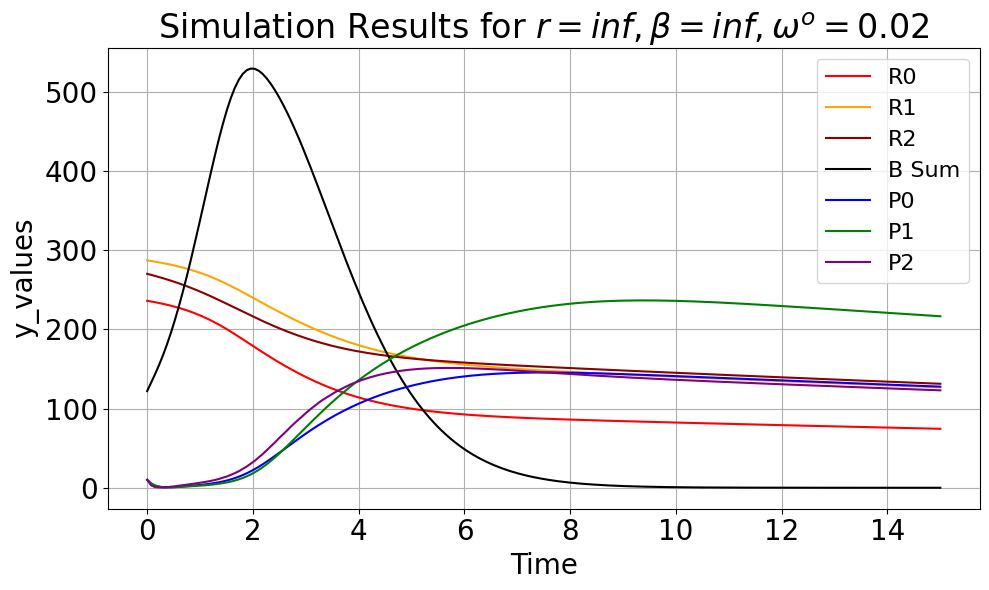
\includegraphics[width=\linewidth]{Images/Plots/Created/UA/r_beta_washout_inf_inf_0.02.png}
        \caption{
            $r, \beta, \omega^o = inf, inf, 0.02$, all initial phage condition=10. 
        }
        \label{fig:created:r_beta_washout_inf_inf_0.02}
    \end{subfigure}
    \caption{
        Varying $r$, $\beta$, and $\omega^o$. 
        All phage values set to 10 to show how the network connections and vector/matrix values affect phage growth. 
        Selectively chosen sub-figures from \Cref{fig:created:r_beta_washout_0}, \Cref{fig:created:r_beta_washout_0.02}, and \Cref{fig:created:r_beta_washout_0.05}. 
        Chosen parameter values can be found in \Cref{tab:appendixE:complex_model}. 
    }
\end{figure}

\section{Phage, Bacteria, and Resource Survivability For a $20\times20\times10$ System}
Finally a large $20\times20\times10$ system can be created